\documentclass[12pt]{article}
\usepackage{amsmath}
\usepackage{amsfonts}
\usepackage{amssymb}
\usepackage{graphicx}
\usepackage{hyperref}
\usepackage{geometry}
\usepackage{amsmath}
\geometry{margin=1in}

\title{Linear Algebra and Differential Equations Project 1}
\author{Rayana Gottschall}
\date{\today}

\begin{document}

\maketitle
\tableofcontents
\newpage

\section{Part 1: Colley Method}
\subsection{Explanation}
Colley's method is used to rank sports teams based on their win-loss ratio.
The method was created by Wesley Colley to handle situations where teams may 
not have played each other an equal number of times. Colley's method takes advantage
of Laplace's Rule of Succession.
\begin{center}
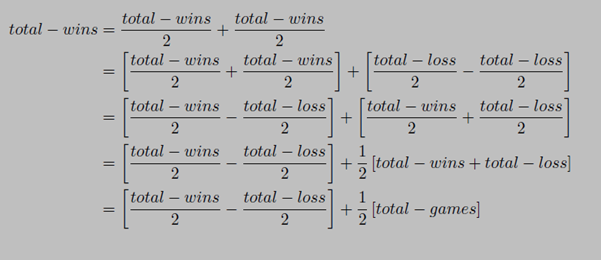
\includegraphics[width=0.8\textwidth]{colleysmethod.png}
\end{center}

\subsection{Laplace's Rule of Succession}
Laplace's Rule of Succession provides a formula to relate observed 
instances to unobserved ones, formally reffered to as "enumerative induction." 
The formula for probability is (k+1)/(n+2). Where 'k' is the number of times an 
event has occured, and 'n' is the total number of trials. 
In sports ranking, Laplace's rule provides a more accurate probabilty result for small data
 sets by accounting for future outcomes. 
This is acheieved through the use of biases, +1 and +2. 
The bias also eases the jumps in ranking when the observed data, number of games played, is
 scarce.


\section{Part 2: Massey Method}
\subsection{Introduction}
Massey's method includes teams' differences in points, and assumes transitivity 
will hold true. The data involved includes a final score differential. And 
a matrix is constructed using the following: 
\newpage
\[
M \cdot r = p
\]
where:
\begin{itemize}
    \item \(\mathbf{M}\): Massey matrix (based on the matchups).
    \item \(\mathbf{r}\): Vector of team ratings (to be solved for).
    \item \(\mathbf{p}\): Vector of point differentials.
\end{itemize}


\subsection{Method of Least Squares}
The method of least squares is used to find a line of best fit for a set of data. 
The goal is to minimize the distance, or error, between the line of best fit 
and the points of data.

\begin{center}
    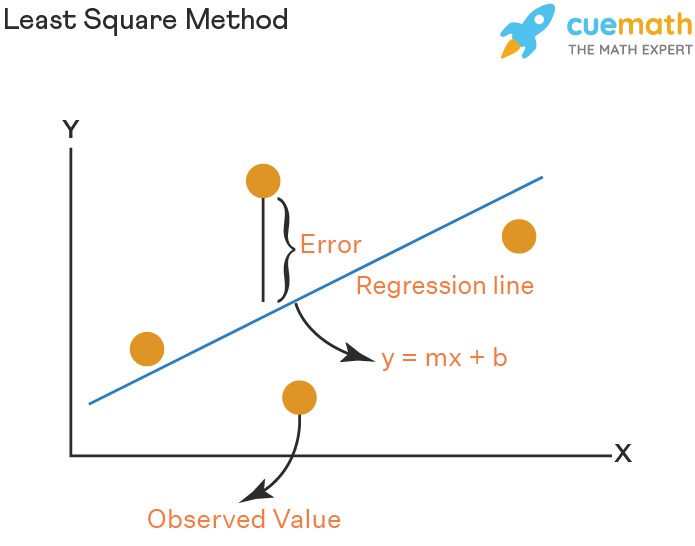
\includegraphics[width=0.8\textwidth]{least-square-method-1-1650276785.png}
    \end{center}


\section{Part 3: Application to Real Data}
In my comparison of Colley's Method and Massey's Method, I used data from the 
2018-2019 NBA season. I found that Colley's method often ranks teams
in a way we'd typically expect, by the W-L ratio. Massey's method is a better 
way to represent team skill based on points scored.

\subsection{Colley's Method Results}
Colley's method gives a team rating between 0 and 1 to indicate performance. 
The lowest rating in my comparision data was Atlanta who went 0-2, and their rating 
was 0.0204. The highest rating was Milwaukee, who went 2-0 in the data set. 
Their rating was 1.0163.

\subsection{Massey's Method Results}
Massey's method gives unbounded rating results to account for performance/score 
differences. The lowest rating was Atlanta again with -22.5. This time the 
highest rating belongs to Charlotte, with a number of 25.833. Despite Charlotte going 1-1 
in the sample data, they took their only win by a great margin. Charlotte beat 
Orlando 120-88.

\section{Part 4: Cutting Edge}
\subsection{Overview of New Methods}
Additional methods to sport rankings include the Elo Rating System, the Bradley-Terry Model,
and Bayesian Analysis. Each method listed has its own unique application. The Elo Rating System 
is primaraily used for chess rankings, but it can be applied to any two player game. 
The Bradley-Terry Method can be used for various team sports and can even be applied to 
election outcomes, among other things. Lastly, the Bayesian Analysis approach is used 
to calculate rankings in motorsport racing.

\subsection{Bayesian Analysis of Formula One Race Results}
Unlike football and basketball, Formula One racing has an additional factor: the car.
Each Formula One team has its own unique car, because of this, in what way can we compare
driver skill? The Bayesian Analysis mathematics proposed by Kesteren and Bergkamp uses driver data 
from 2014-2021 and the attributes are as follows: driver id, constructor id, season, race number, 
finishing position, and status. Additional race information included weather conditions (ie wet 
or dry) and circuit type (street or permanent).

\subsubsection{Diving into the Math}
For each race, r, we assume there is a set of competitors, C. The outcome is a vector which 
represents a ranking of competitors, y. The ranking follows a Rank-Ordered Logit model where 
finish position (ranking) is modeled as a function of driver skill, constructor advantage, and 
yearly variations in performance.

Rank-Ordered Logit:
\[
\mathbf{y}_r \sim \text{RankOrderedLogit}(\boldsymbol{\theta}_r)
\]
where \(\boldsymbol{\theta}_r\) represents the latent abilities of competitors in race \(r\).

Latent Ability Decomposition: 
the ability of a competitor is decomposed into the following components
\[
\theta_c = \theta_d + \theta_{ds} + \theta_t + \theta_{ts}
\]
\[
\begin{aligned}
&\theta_d \text{: Long-term driver skill,} \\
&\theta_{ds} \text{: Seasonal deviation of driver skill,} \\
&\theta_t \text{: Long-term constructor advantage,} \\
&\theta_{ts} \text{: Seasonal deviation of constructor advantage.}
\end{aligned}
\]



\begin{center}
    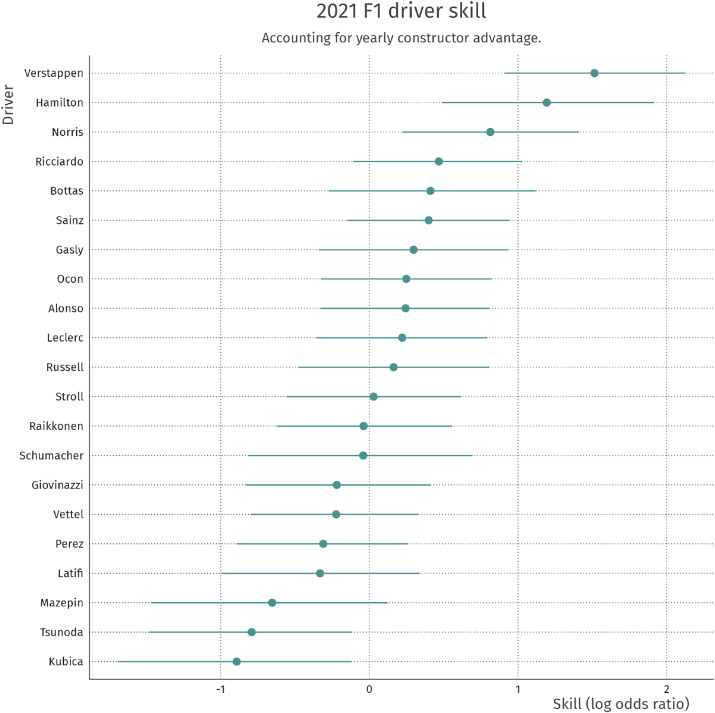
\includegraphics[width=0.8\textwidth]{driver skill.jpg}
    \end{center}
The figure above depicts overall driver skill, taking the car model into account.

\newpage
\section*{References}
\begin{flushleft}
The Elo System:

https://compass.blogs.bristol.ac.uk/2020/12/17/the-elo-rating-system-from-chess-to-education/

Bayesian Analysis:

https://pmc.ncbi.nlm.nih.gov/articles/PMC10660124/

Laplace's Rule of Sucession:

https://jonathanweisberg.org/post/inductive-logic-2/

Method of Least Squares:
https://www.investopedia.com/terms/l/least-squares-method.asptext=The%20least%20squares%20method%20is%20a%20statistical%20procedure%20to%20find,the%20behavior%20of%20dependent%20variables.
\end{flushleft}
\end{document}
